\documentclass[10pt,dvipsnames]{beamer}

\definecolor{links}{HTML}{2A1B81}
\hypersetup{colorlinks,linkcolor=,urlcolor=links}

\usetheme{metropolis}
\metroset{block=fill}
%\setmonofont{Ubuntu Mono}

\usepackage{appendixnumberbeamer}

\usepackage{booktabs,empheq,bbold,bm}
\usepackage[scale=2]{ccicons}

\usepackage{pgfplots}
\usepgfplotslibrary{dateplot}

\usepackage{xspace}
\newcommand{\themename}{\textbf{\textsc{metropolis}}\xspace}

% for python listings; inspired by https://gist.github.com/YidongQIN/a10dd4f72381362aff4257e7a5541d86 
\usepackage{listings}
\usepackage{color}
\definecolor{darkred}{rgb}{0.6,0.0,0.0}
\definecolor{darkgreen}{rgb}{0,0.50,0}
\definecolor{lightblue}{rgb}{0.0,0.42,0.91}
\definecolor{orange}{rgb}{0.99,0.48,0.13}
\definecolor{grass}{rgb}{0.18,0.80,0.18}
\definecolor{pink}{rgb}{0.97,0.15,0.45}
\lstdefinelanguage{PythonPlus}[]{Python}{
  morekeywords=[1]{,as,assert,nonlocal,with,yield,self,True,False,None,} % Python builtin
  morekeywords=[2]{,__init__,__add__,__mul__,__div__,__sub__,__call__,__getitem__,__setitem__,__eq__,__ne__,__nonzero__,__rmul__,__radd__,__repr__,__str__,__get__,__truediv__,__pow__,__name__,__future__,__all__,}, % magic methods
  morekeywords=[3]{,object,type,isinstance,copy,deepcopy,zip,enumerate,reversed,list,set,len,dict,tuple,range,xrange,append,execfile,real,imag,reduce,str,repr,}, % common functions
  morekeywords=[4]{,Exception,NameError,IndexError,SyntaxError,TypeError,ValueError,OverflowError,ZeroDivisionError,}, % errors
  morekeywords=[5]{,ode,fsolve,sqrt,exp,sin,cos,arctan,arctan2,arccos,pi, array,norm,solve,dot,arange,isscalar,max,sum,flatten,shape,reshape,find,any,all,abs,plot,linspace,legend,quad,polyval,polyfit,hstack,concatenate,vstack,column_stack,empty,zeros,ones,rand,vander,grid,pcolor,eig,eigs,eigvals,svd,qr,tan,det,logspace,roll,min,mean,cumsum,cumprod,diff,vectorize,lstsq,cla,eye,xlabel,ylabel,squeeze,}, % numpy / math
}
\lstdefinestyle{colorEX}{
  basicstyle=\ttfamily\small,
  backgroundcolor=\color{white},
  commentstyle=\color{darkgreen}\slshape,
  keywordstyle=\color{blue}\bfseries\itshape,
  keywordstyle=[2]\color{blue}\bfseries,
  keywordstyle=[3]\color{grass},
  keywordstyle=[4]\color{red},
  keywordstyle=[5]\color{orange},
  stringstyle=\color{darkred},
  emphstyle=\color{pink}\underbar,
}
\lstset{style=colorEX,
        basewidth = {.49em}}

\newcommand{\bg}{\mathbf{g}}
\newcommand{\bn}{\mathbf{n}}
\newcommand{\bq}{\mathbf{q}}
\newcommand{\bu}{\mathbf{u}}

\newcommand{\bU}{\mathbf{U}}

\newcommand{\bzero}{\bm{0}}

\newcommand{\eps}{\epsilon}
\newcommand{\grad}{\nabla}
\newcommand{\Div}{\nabla\cdot}

\newcommand{\rhoi}{\rho_{\text{i}}}
\newcommand{\snew}{s^{\text{new}}}

\newcommand{\comm}[1]{{\footnotesize \hfill \emph{#1}}}


\title{A space-time view of good glacier models}
%\subtitle{version 1.0}
\date{NWG 2024}
\author{Ed Bueler}
\institute{University of Alaska Fairbanks}
%\titlegraphic{\vspace{-1cm}\par\hspace{-1cm}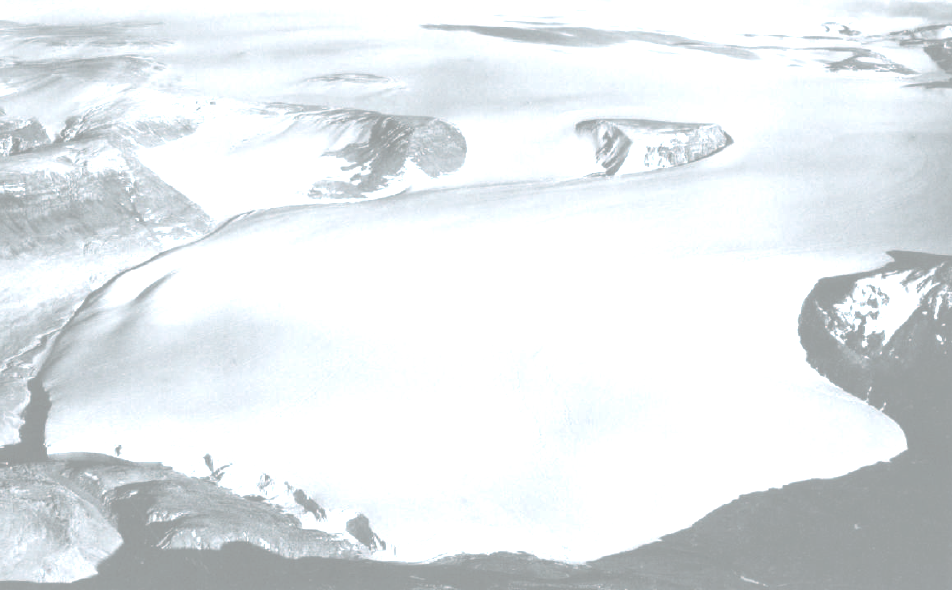
\includegraphics[width=1.5\textwidth]{polaris-overexposed.png}}

\begin{document}
\graphicspath{{figs/}}

\maketitle

%\begin{frame}{Outline}
  %\setbeamertemplate{section in toc}[sections numbered]
  %\tableofcontents[hideallsubsections]
  %\tableofcontents
%\end{frame}


%\section[how does the glacier surface move?]{\textbf{how does the glacier surface move?} (hour 1)}
%\subsection{basic mathematics}


\begin{frame}{only a view point}

\begin{itemize}
\item this is an informal view-point talk
\item not a results talk
%\item vaguely about my recent work
\end{itemize}
\end{frame}


\begin{frame}{common goals}

I am assuming certain goals/attitudes in common with this audience:
\begin{enumerate}
\item we care about how the glaciated area evolves in a numerical model
\item good glacier models need to balance membrane/longitudinal stresses
%\item simulation speed at a given spatial resolution is what matters
\end{enumerate}
\end{frame}


\begin{frame}{the life of a glacier in space-time}

\bigskip
\hfill 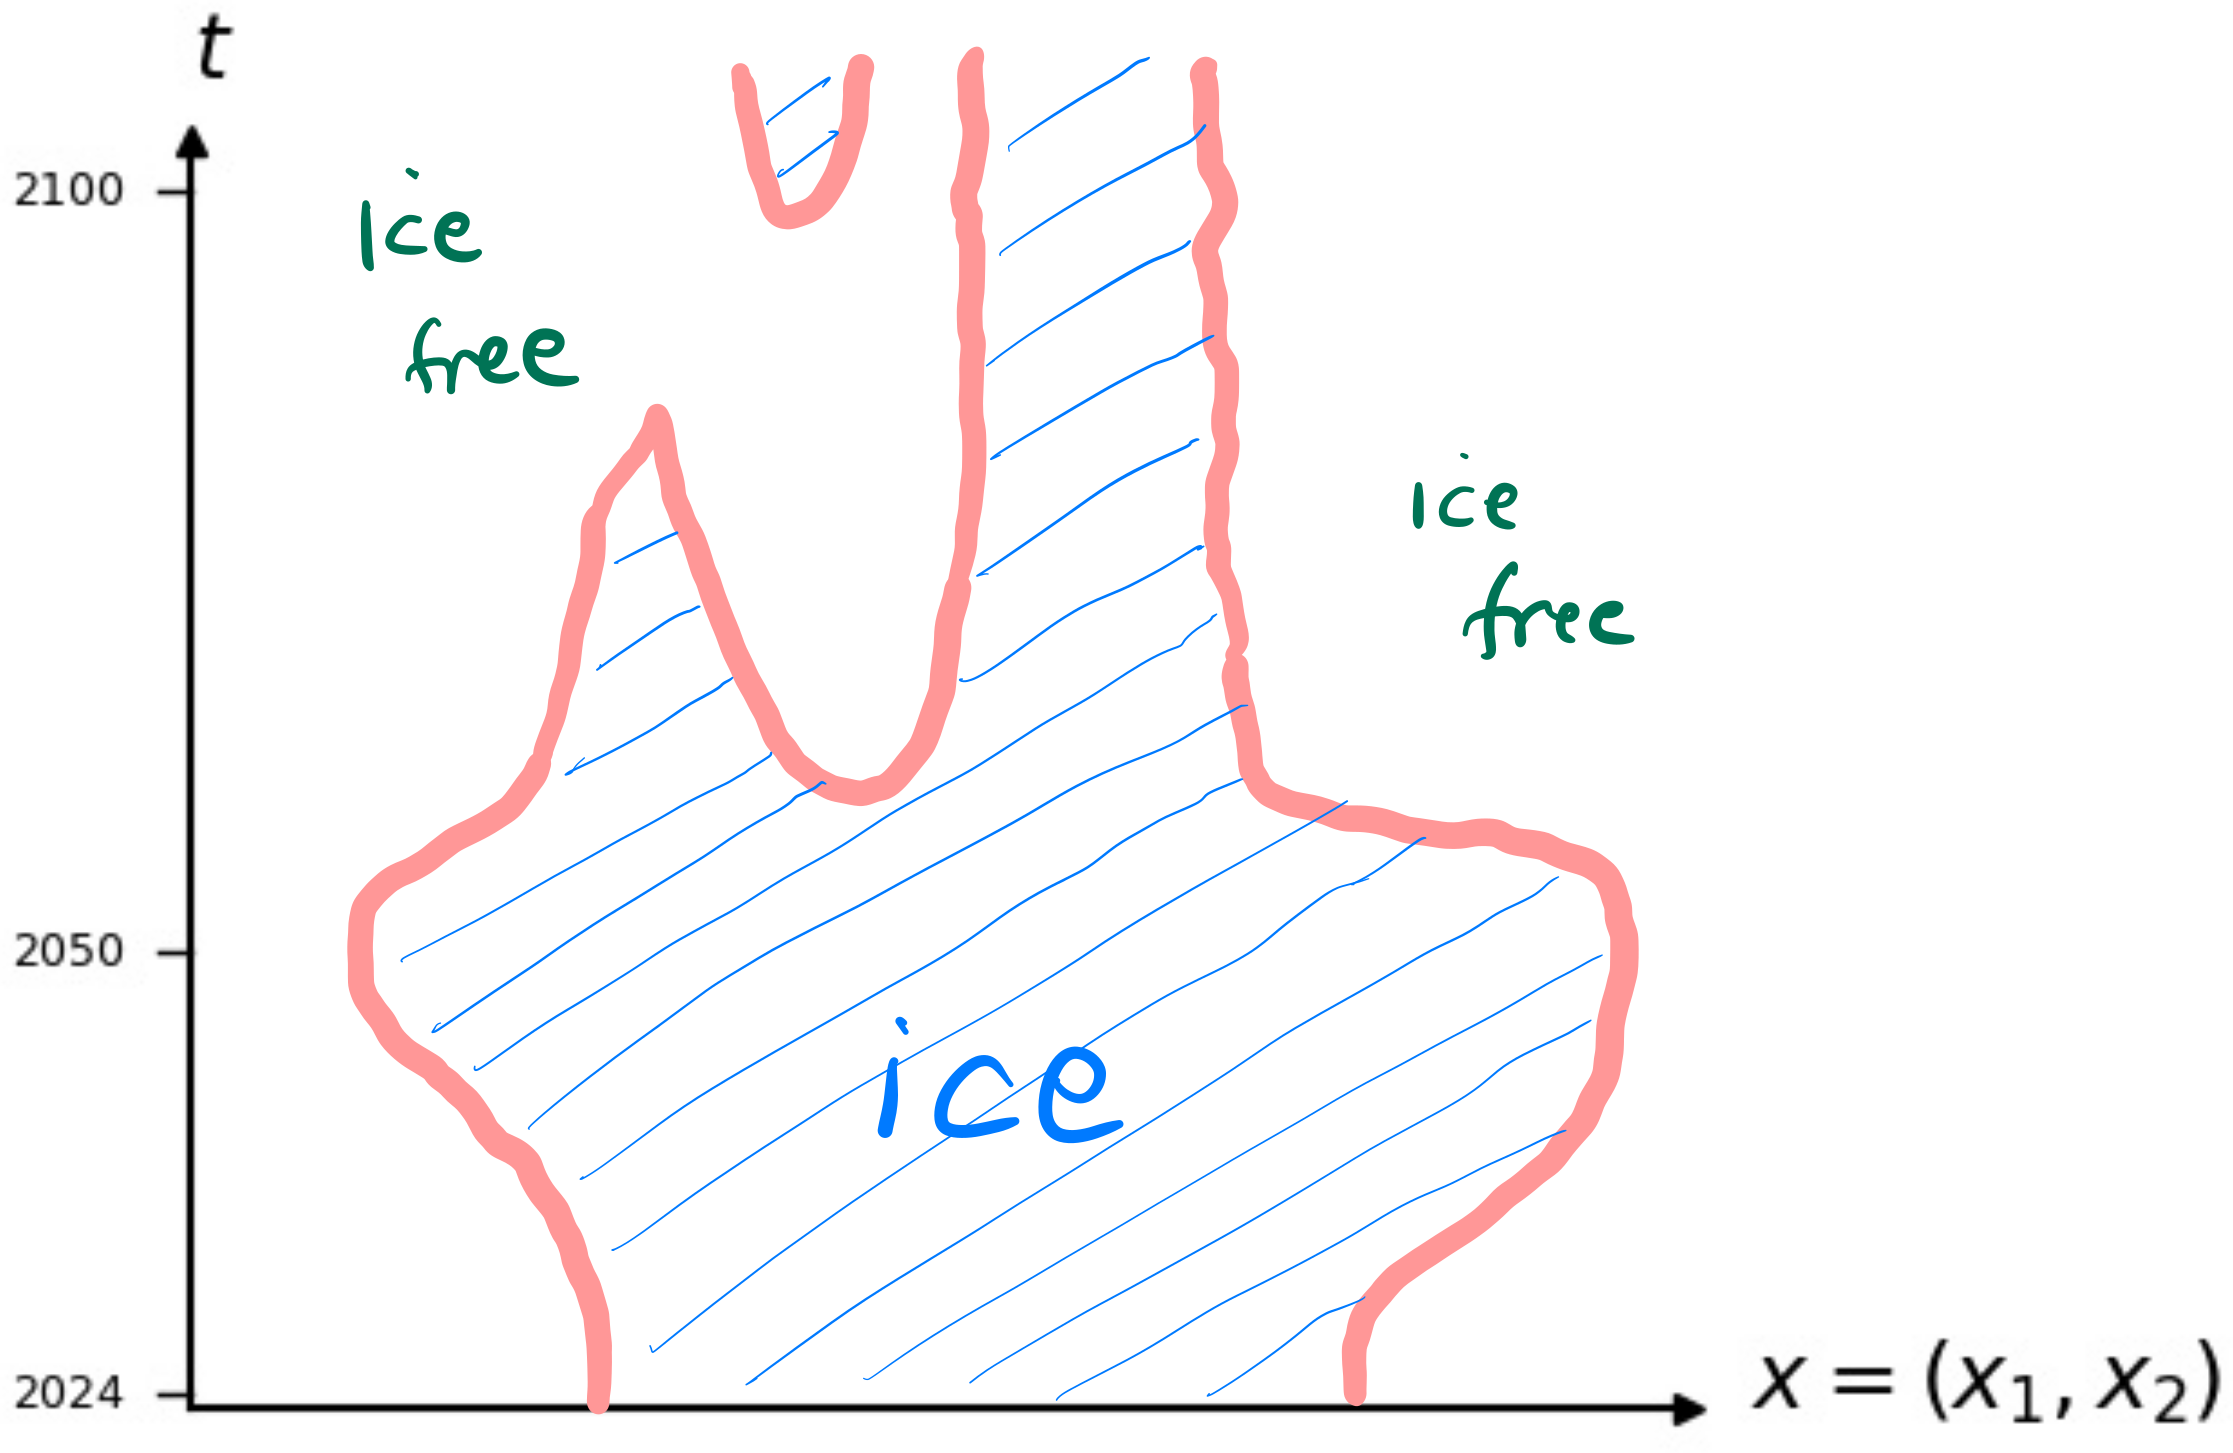
\includegraphics[width=\textwidth]{xtcartoon}
\end{frame}


\begin{frame}{\underline{the} 3 views}

\begin{center}
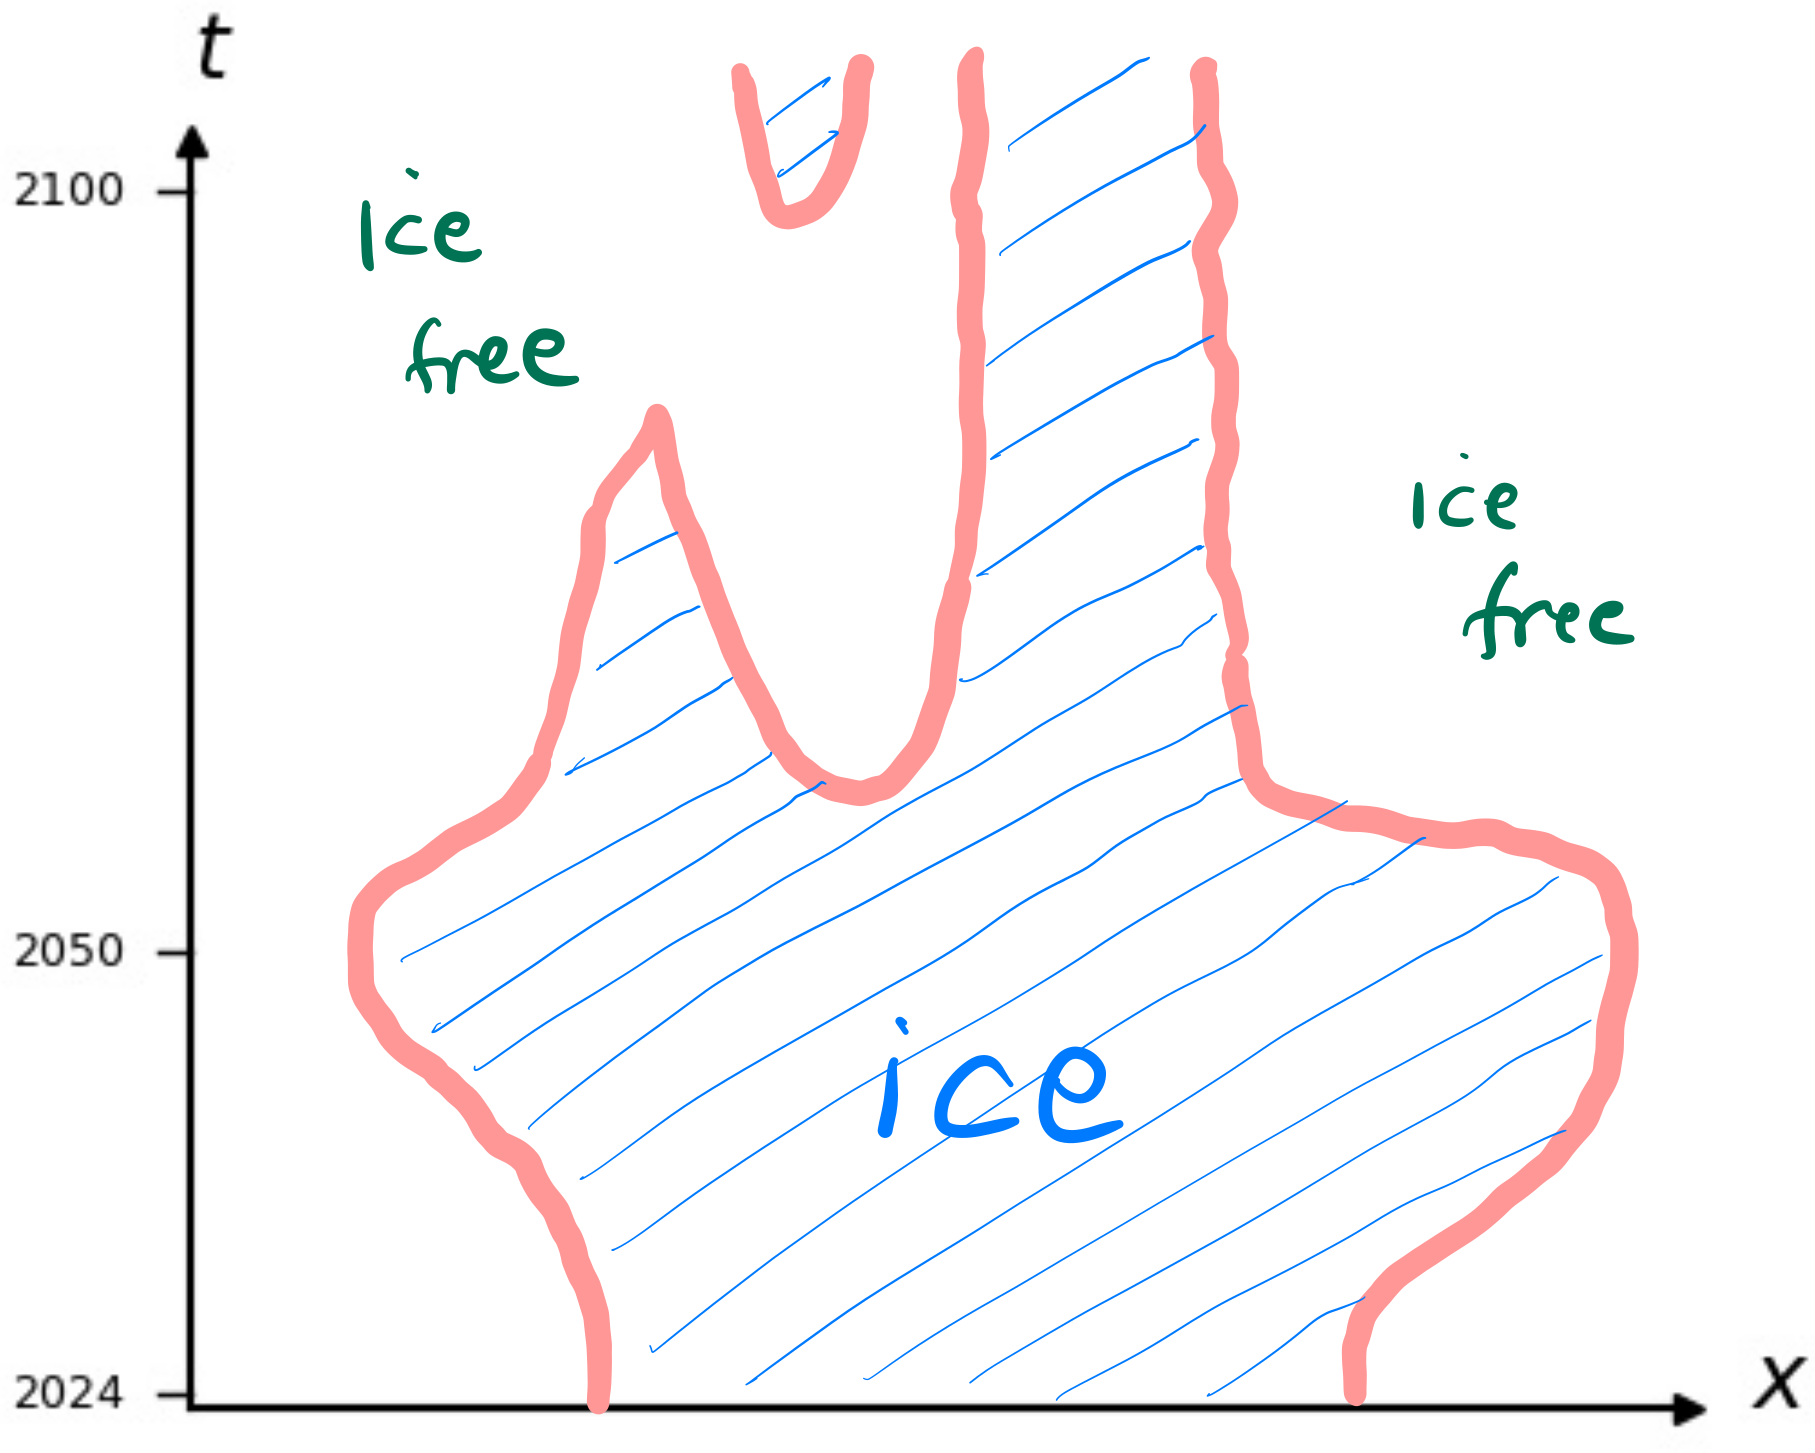
\includegraphics[width=0.5\textwidth]{xtcrop}
\end{center}

\begin{columns}
\begin{column}{0.45\textwidth}
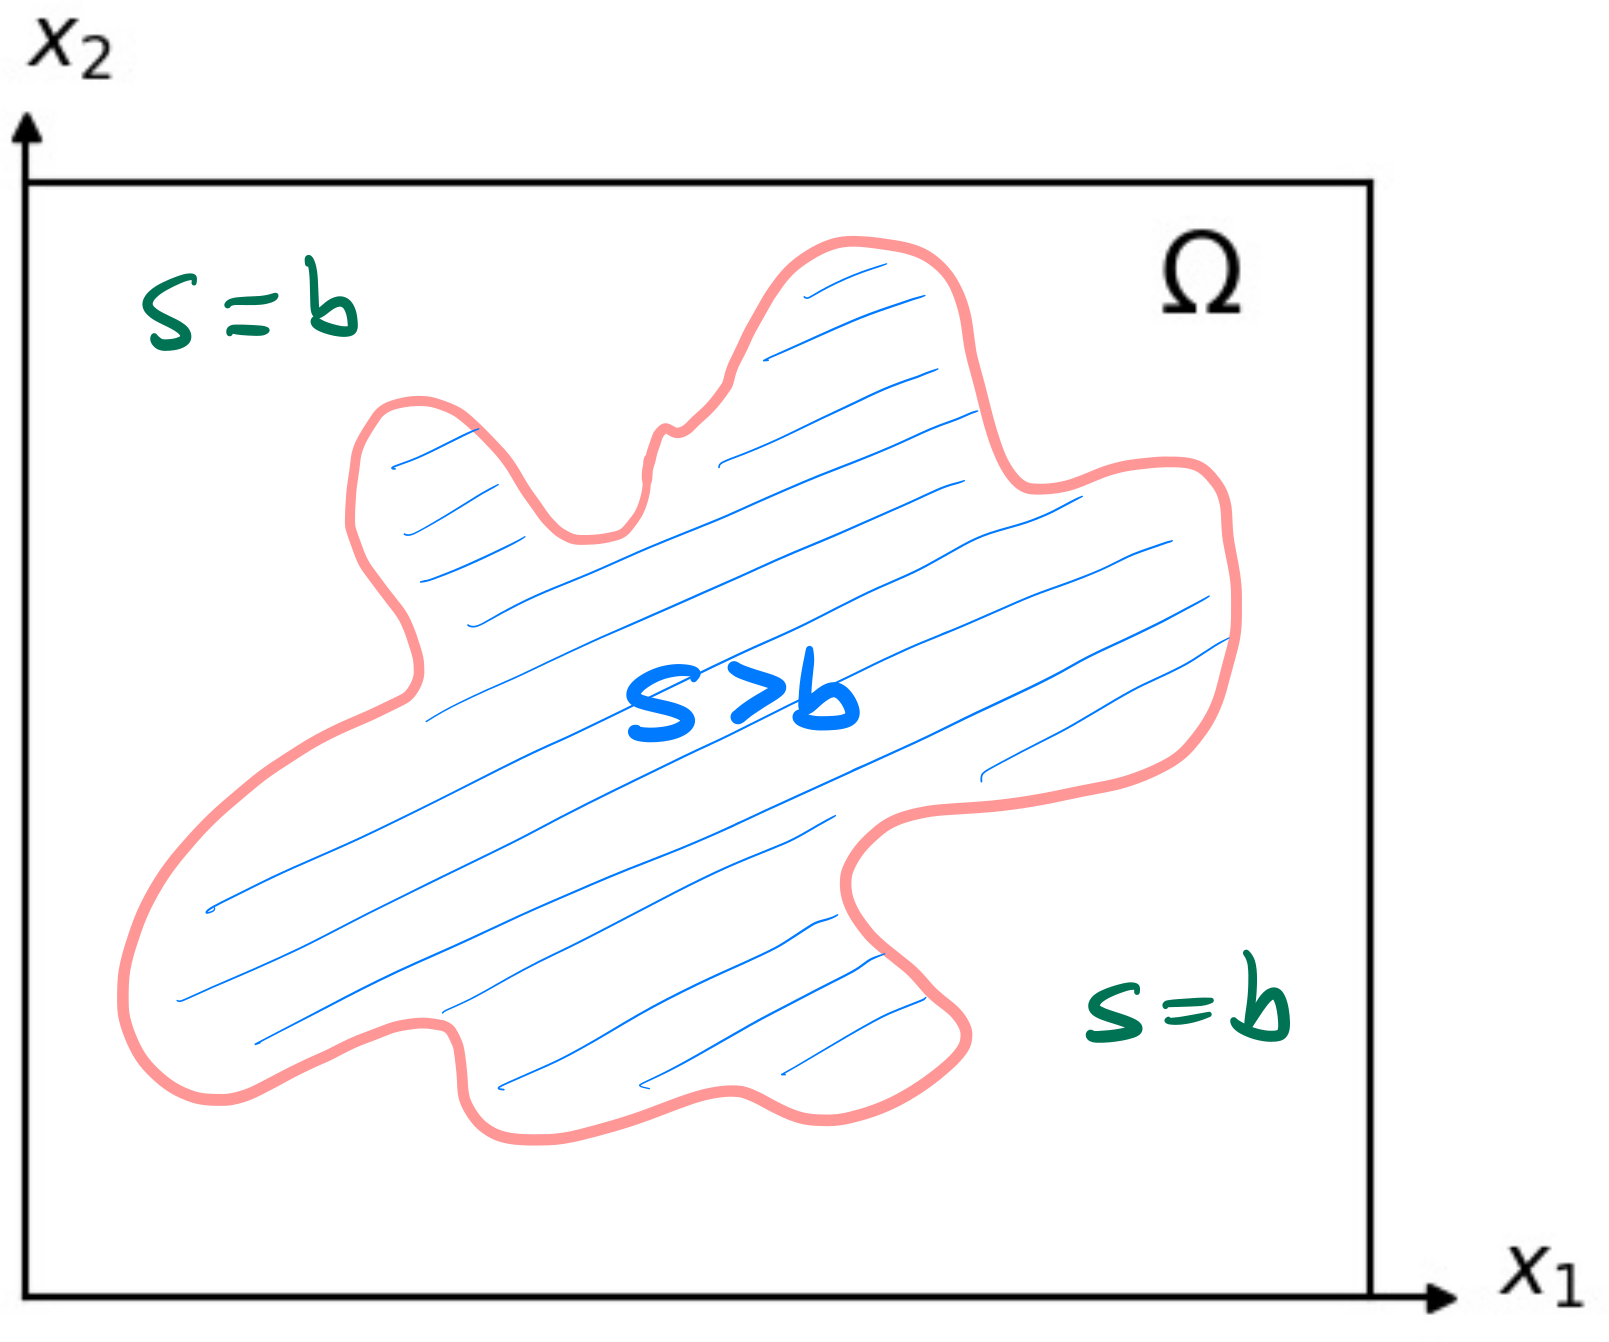
\includegraphics[width=0.8\textwidth]{mapplane}
\end{column}
\begin{column}{0.55\textwidth}
\hfill 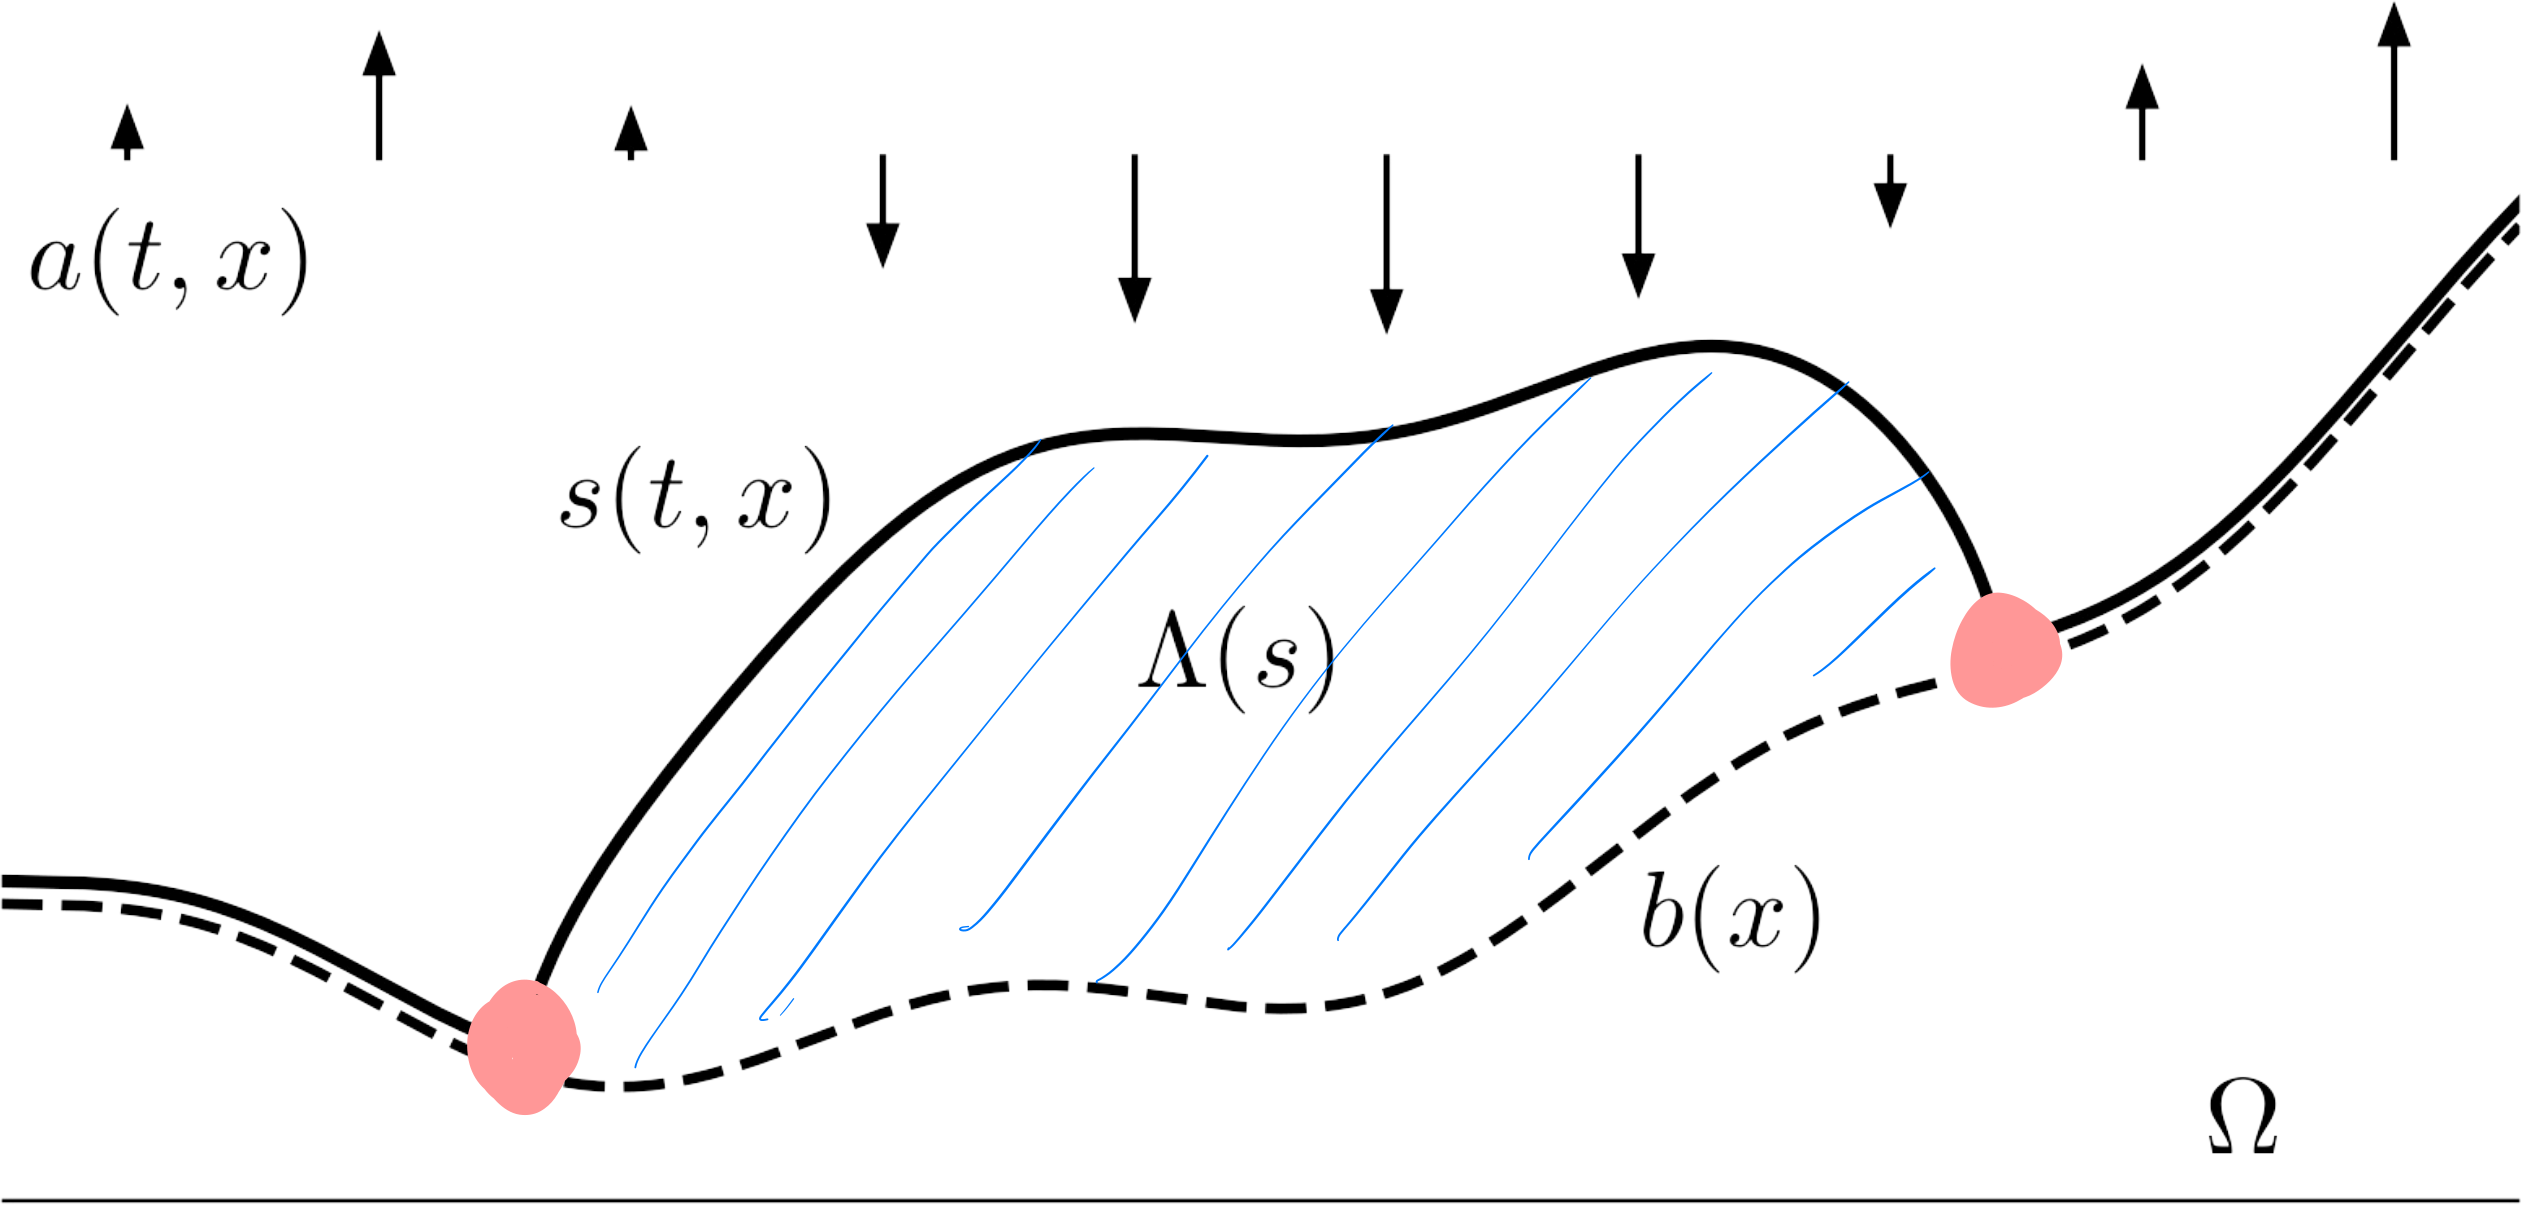
\includegraphics[width=\textwidth]{stokesdomainpink}
\end{column}
\end{columns}
\end{frame}


\newcommand{\where}[1]{\text{\footnotesize #1}}

\begin{frame}{\underline{the} (viscous) mathematical model}

\begin{align*}
s - b &\ge 0 & &\where{in $\Omega$} \\
\frac{\partial s}{\partial t} - \bu|_s \cdot \bn_s - a &\ge 0 & &\where{in $\Omega$} \\
(s - b) \left(\frac{\partial s}{\partial t} - \bu|_s \cdot \bn_s - a\right) &= 0 & &\where{in $\Omega$} \\
- \nabla \cdot \left(2 \nu(D\bu)\, D\bu\right) + \nabla p &= \rhoi \bg && \where{in $\Lambda(s)$} \\
\nabla \cdot \bu &= 0 && \where{in $\Lambda(s)$} \\
\nu(D\bu) &= \nu_n \left(|D\bu|^2 + \eps\right)^{q_n} && \where{in $\Lambda(s)$} \\
\left(2 \nu(D\bu) D\bu - pI\right) \bn_s &= \bzero && \where{on $\Gamma_s \subset \partial\Lambda(s)$} \\
\bu  = \bzero \text{ } &\text{or } f(\bu,D\bu)=0 && \where{on $\Gamma_b \subset \partial\Lambda(s)$}
\end{align*}
\end{frame}


\newcommand{\viewin}[1]{{\footnotesize \emph{this view appears in} #1}}

\begin{frame}{what is true at different points $(t,x)$?}

\bigskip \bigskip

\begin{columns}
\begin{column}{0.26\textwidth}
\begin{itemize}
\item[a)] what is \emph{true} in the ice?
\item[b)] what is \emph{true} on bare land?
\item[c)] what is \emph{true} at the free boundary?
\end{itemize}\end{column}
\begin{column}{0.74\textwidth}
\hfill 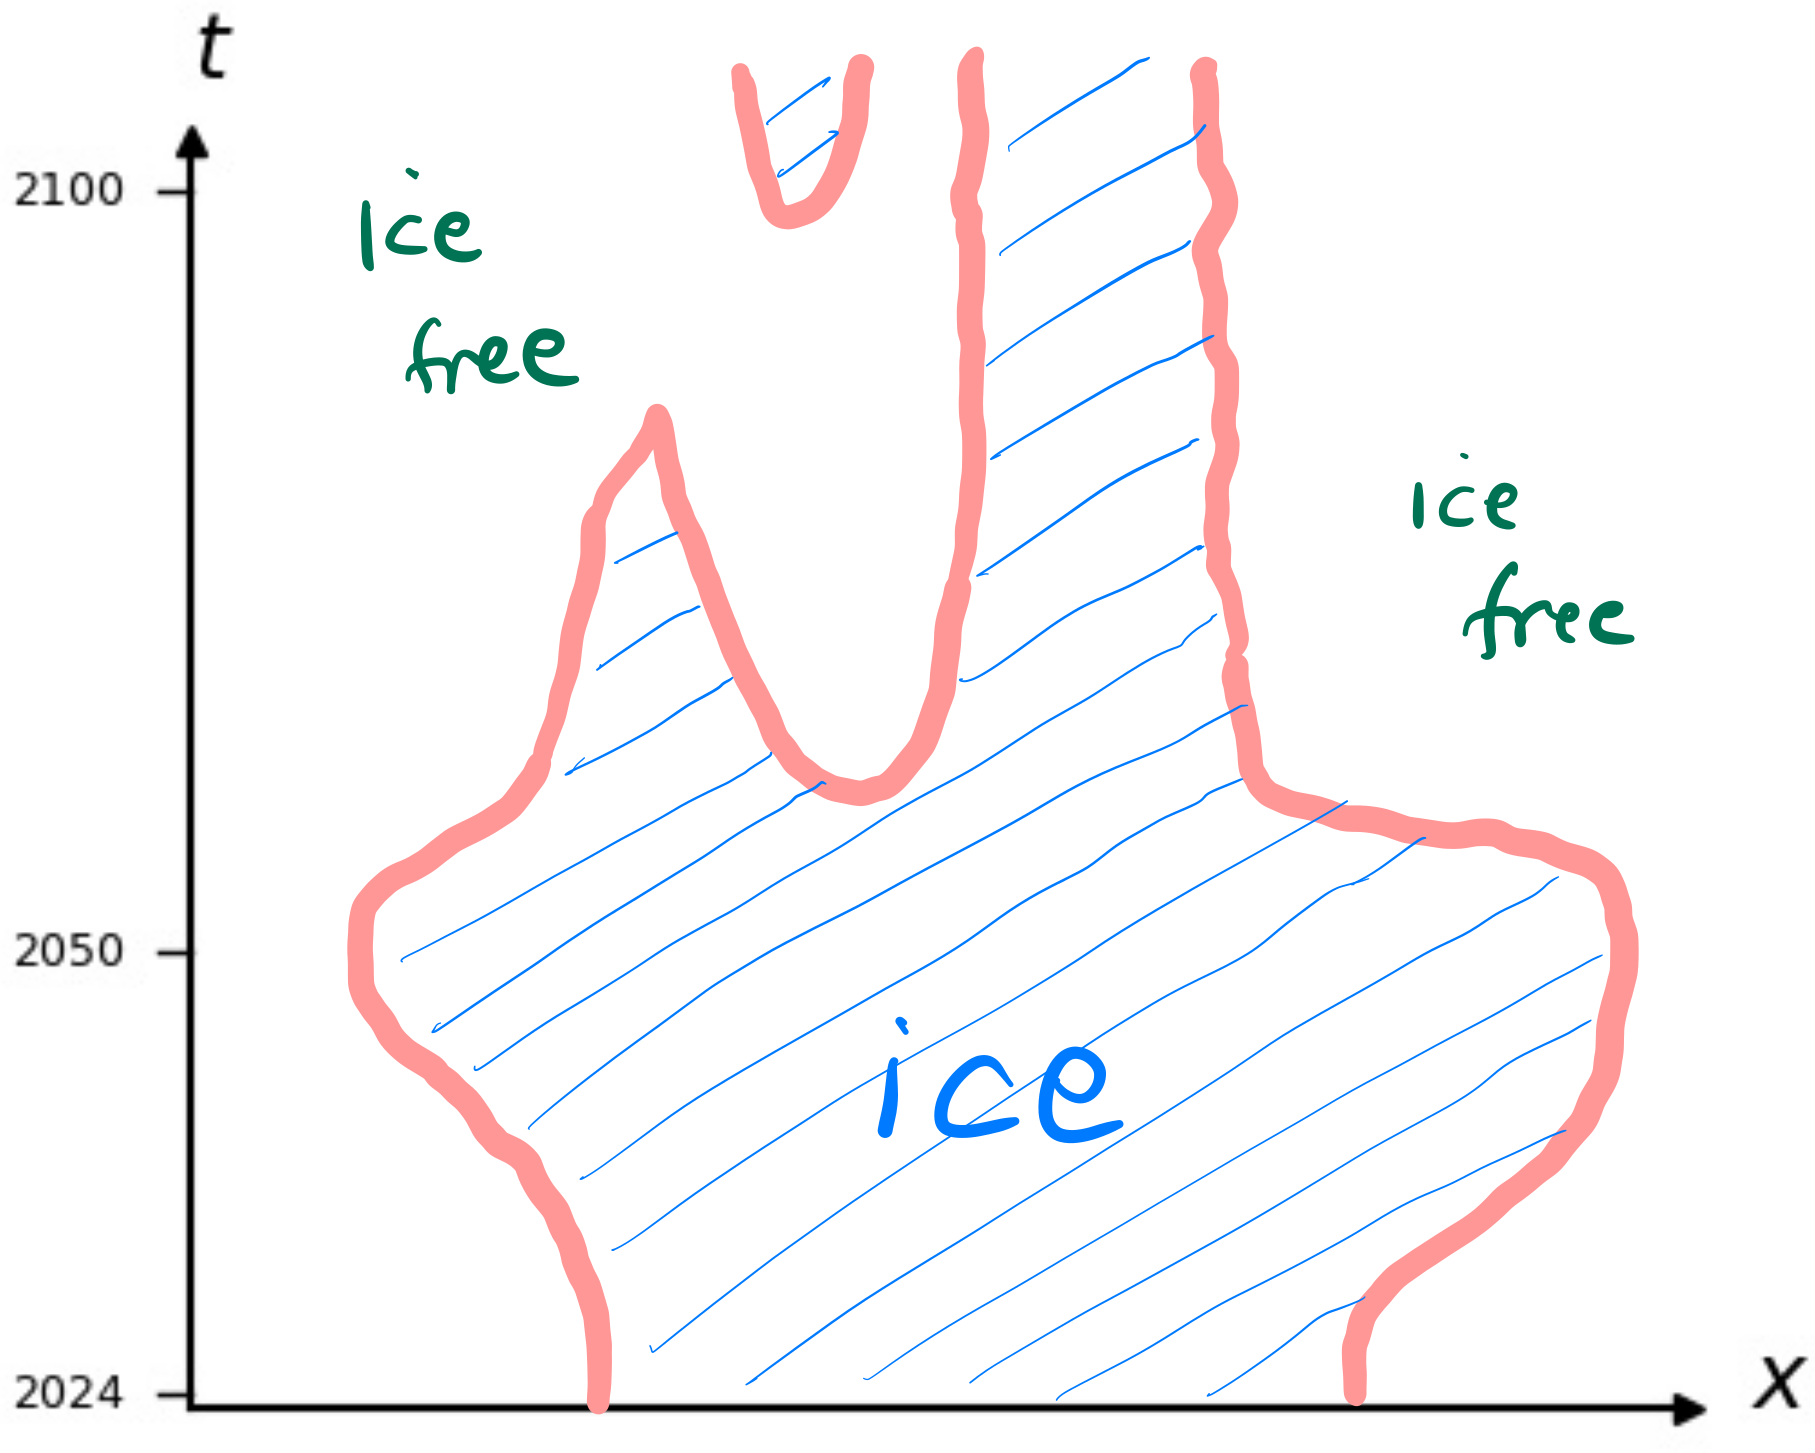
\includegraphics[width=\textwidth]{xtcrop}
\end{column}
\end{columns}
\end{frame}


\begin{frame}{what is true \alert{everywhere} in $\Omega$?}

\hfill 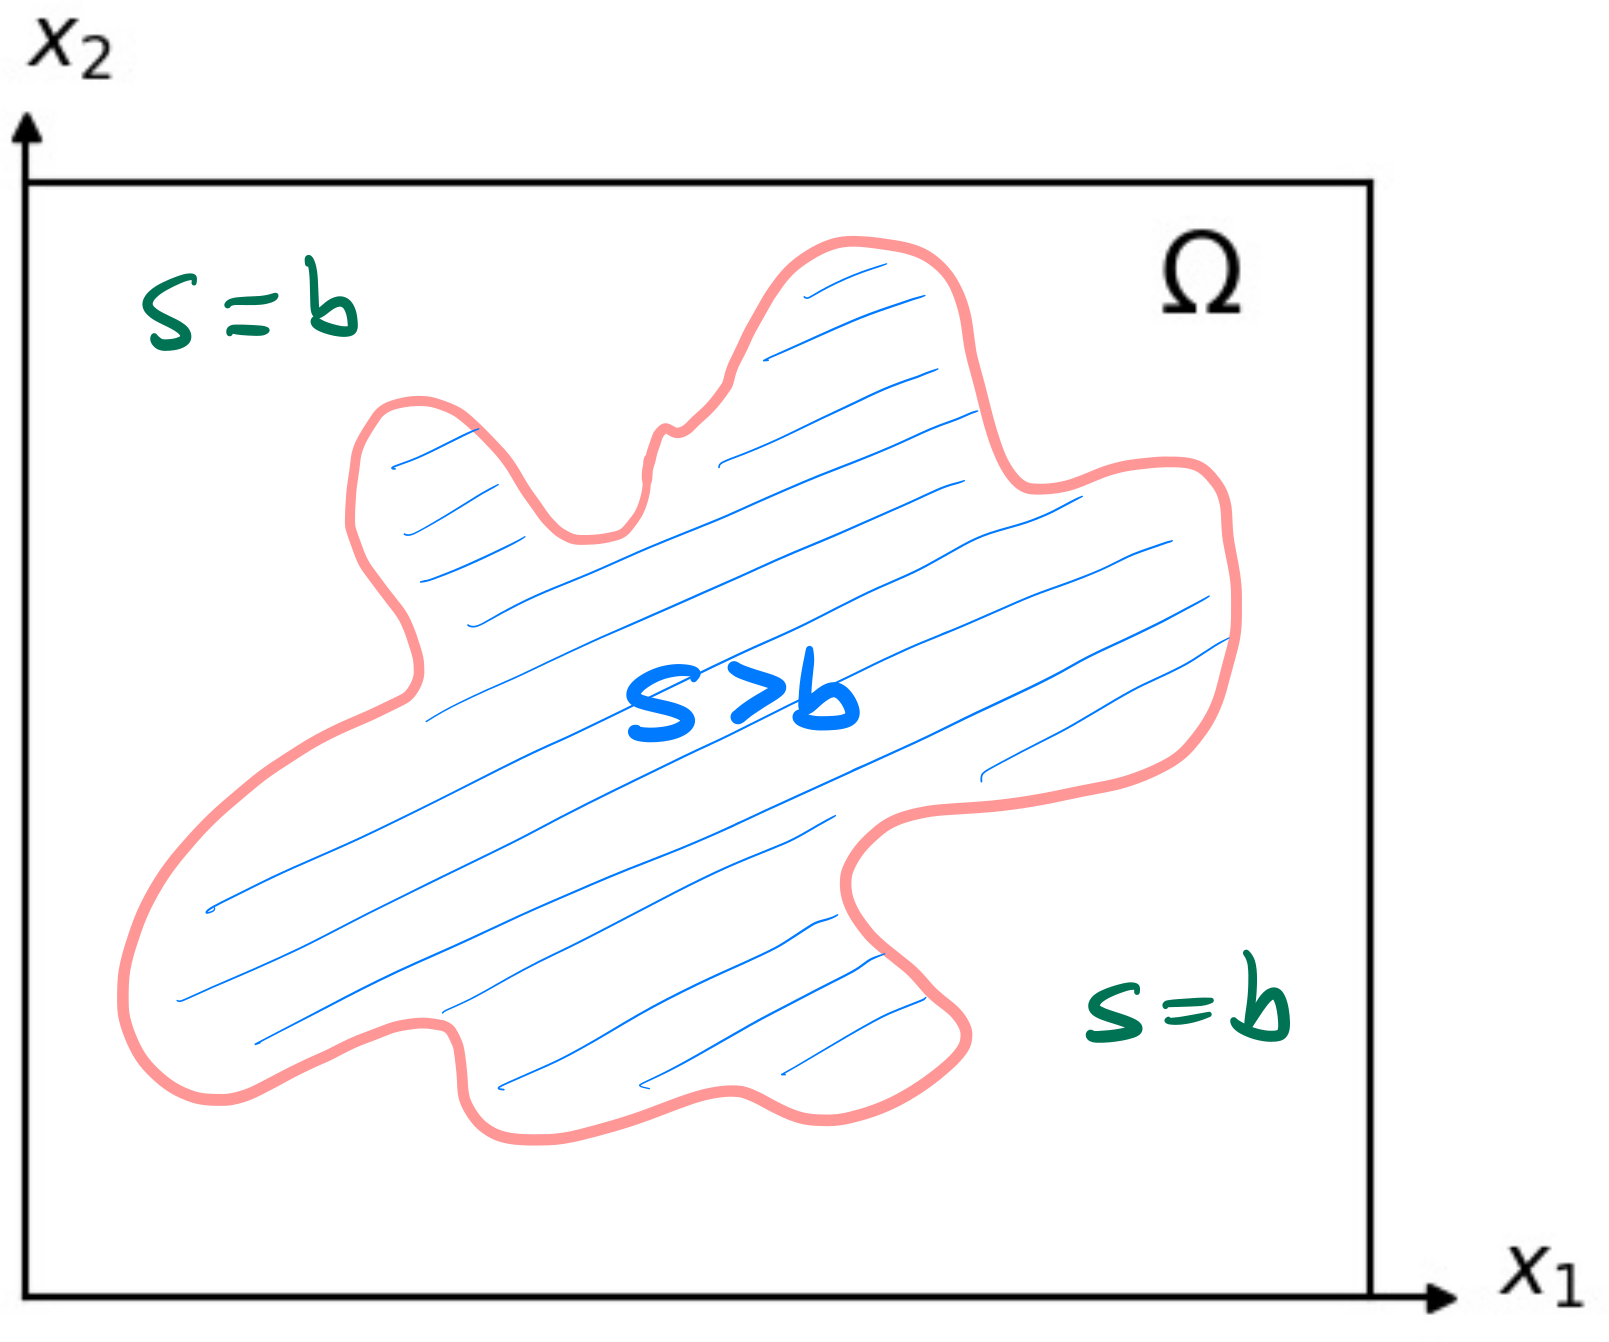
\includegraphics[width=0.35\textwidth]{mapplane}

\begin{align*}
s - b &\ge 0 & &\where{in $\Omega$} \\
\frac{\partial s}{\partial t} - \bu|_s \cdot \bn_s - a &\ge 0 & &\where{in $\Omega$} \\
(s - b) \left(\frac{\partial s}{\partial t} - \bu|_s \cdot \bn_s - a\right) &= 0 & &\where{in $\Omega$}
\end{align*}

\vspace{10mm}
{\footnotesize \emph{this nonlinear complementarity problem first appears in (Calvo et al 2003), \emph{for SIA}}}
\end{frame}


\begin{frame}{result (and last slide): an FE error theorem}

\begin{itemize}
\item you will be disappointed: ``result'' here means a theorem about size of finite element (FE) errors
\item this theorem needs ``reasonable'' assumptions for a (continuum) geometry- evolving, Stokes model for glaciers \dots including \textbf{conjectured} well-posedness
\item \emph{Theorem (Bueler, 2024).}  the FE error in computing an updated surface elevation, using an implicit time step, comes from 3 terms:
\begin{align*}
\|s_h-s\|^r &\le \quad \frac{c_1}{\Delta t} \int_{\Omega_A(s)} (b - \ell) (b_h - b) \\
   &\quad\, + \Gamma \big\|\bu_h - \bu\big\| \\
   &\quad\, + c_0 \|\Pi_h(s) - s\|^q
\end{align*}
\item this separates the causes of surface elevation errors:
    \begin{enumerate}
    \item discretizing the bed elevation ($b_h$ versus exact $b$)
    \item numerically solving the Stokes equations ($\bu_h$ versus exact $\bu$)
    \item Cea's lemma for the surface elevation ($s_h$ versus exact $s$) \strut
        \begin{itemize}
        \item[$\circ$] $s$ necessarily projected to be admissible with respect to $b_h$
        \end{itemize}
    \end{enumerate}
\end{itemize}
\end{frame}


\begin{frame}{conclusion}

\begin{itemize}
\item thank you for listening!
\item I'll appreciate any help I can get \dots
\end{itemize}
\end{frame}


\begin{frame}{references}

{\footnotesize % inputed at end of slides.tex

\newcommand{\sdoi}[1]{\,{\scriptsize \href{https://doi.org/#1}{doi:#1}}}
\newcommand{\surl}[2]{\,{\scriptsize \href{#1}{#2}}}

\begin{itemize}
%\item E.~Bueler (2021). \emph{Conservation laws for free-boundary fluid layers}, SIAM J.~Appl.~Math.~81 (5), 2007--2032 \sdoi{10.1137/20M135217X}
%\item E.~Bueler (2022). \emph{Performance analysis of high-resolution ice-sheet simulations}, J.~Glaciol.~69 (276), 930--935 \sdoi{10.1017/jog.2022.113}
%\item E.~Bueler \& P.~Farrell (2024).  \emph{A full approximation scheme multilevel method for nonlinear variational inequalities}, SIAM J.~Sci.~Comput.~46 (4), \sdoi{10.1137/23M1594200}
\item E.~Bueler (2024). \emph{Surface elevation errors in finite element {S}tokes models for glacier evolution}, submitted \surl{https://arxiv.org/abs/2408.06470}{arxiv:2408.06470}
\item N.~Calvo and others (2003). \emph{On a doubly nonlinear parabolic obstacle problem modelling ice sheet dynamics}, SIAM J.~Appl.~Math.~63 (2), 683--707 \sdoi{10.1137/S0036139901385345}
%\item T.~Isaac, G.~Stadler, \& O.~Ghattas (2015). \emph{Solution of nonlinear Stokes equations \dots ice sheet dynamics}, SIAM J.~Sci.~Comput., 37 (6), B804--B833 \sdoi{10.1137/140974407}
%\item G.~Jouvet \& E.~Bueler (2012). \emph{Steady, shallow ice sheets as obstacle problems: well-posedness and finite element approximation}, SIAM J.~Appl.~Math.~72 (4), 1292--1314 \sdoi{10.1137/110856654}
\item G.~Jouvet \& J.~Rappaz (2011). \emph{Analysis and finite element approximation of a nonlinear stationary {S}tokes problem \dots}, Adv.~Numer.~Analysis 2011 (164581) \sdoi{10.1155/2011/164581}
%\item A.~L{\"o}fgren, J.~Ahlkrona \& C. Helanow (2022). \emph{Increasing stable time-step sizes of the free-surface problem arising in ice-sheet simulations},~J. Comput. Phys.: X 16 (100114) \sdoi={10.1016/j.jcpx.2022.100114}
\end{itemize}
}
\end{frame}


\begin{frame}[standout]

extra slides
\end{frame}


\begin{frame}{3 benefits of the space-time view}

\begin{enumerate}
\item \alert{(numerical time-stepping)} you can see \emph{what ``fully-implicit'' must mean}
\item \alert{(practical modeling)} you can see \emph{why modeled surface mass balance must be available on space \& time adjacent ice-free land}
\item \alert{(mathematical ignorance)} you can consider \emph{what determines the evolution of the glaciated area}, and how unclear that is at present
\end{enumerate}

\end{frame}


\begin{frame}{benefit 1: numerical time-stepping}

what does ``fully-implicit'' time-stepping mean?

\medskip

\begin{center}
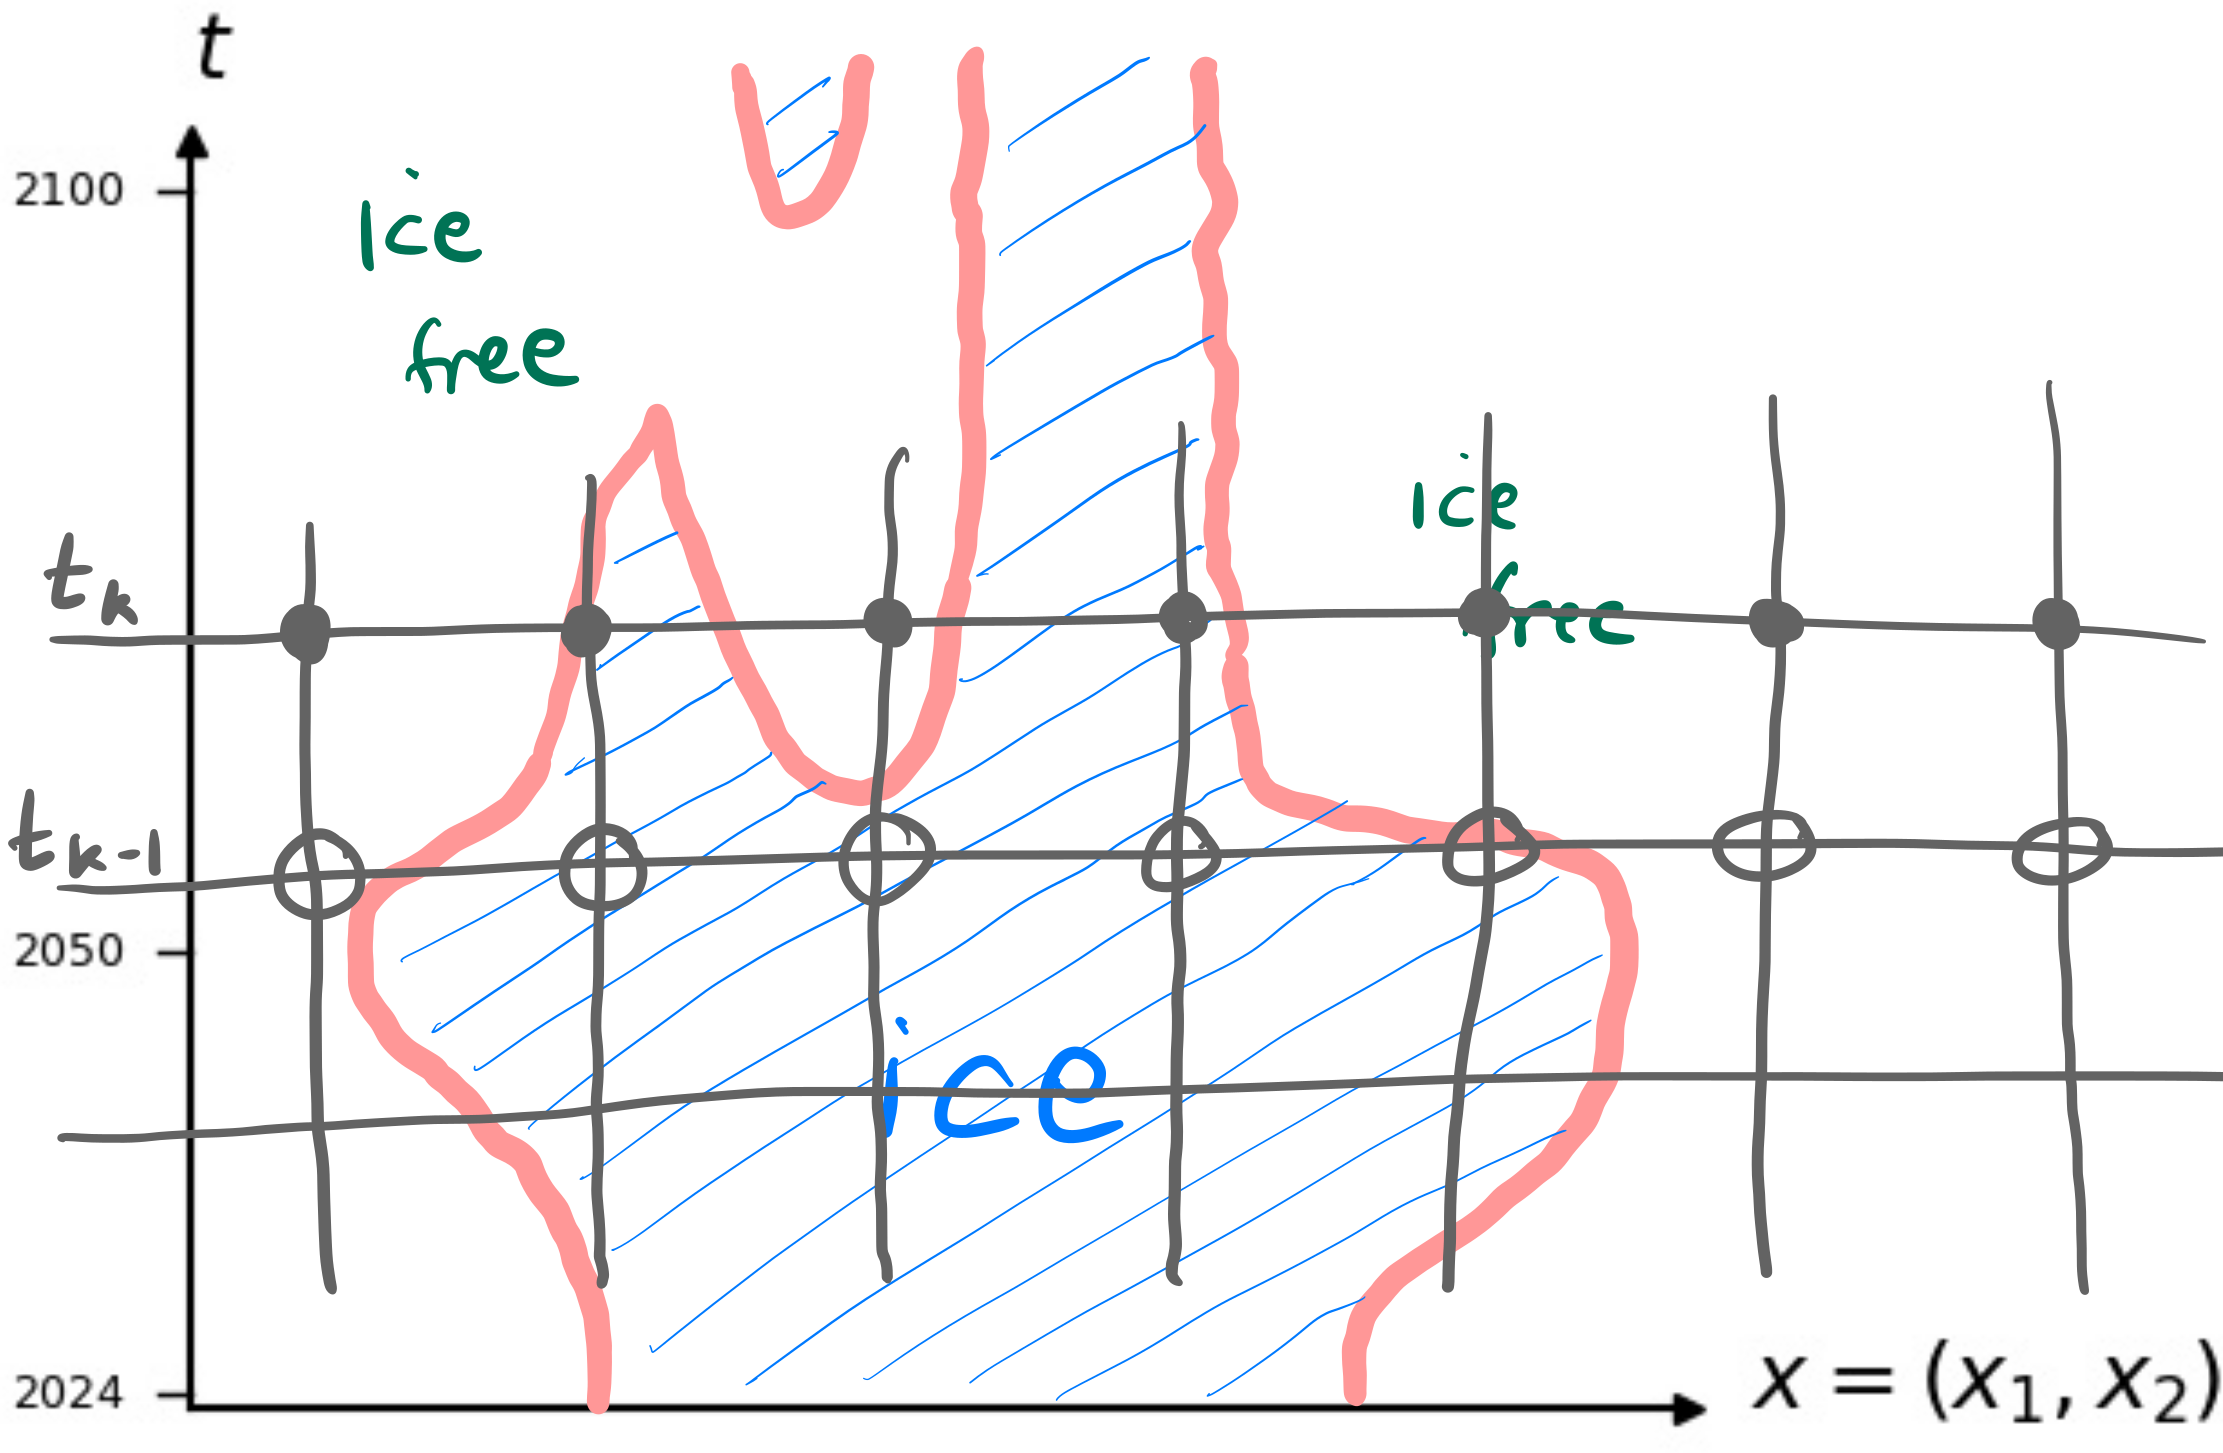
\includegraphics[width=0.8\textwidth]{implicitstep}
\end{center}

\medskip
\viewin{(Bueler, 2022)}

{\footnotesize \emph{note appealing semi-implicit idea in} (L\"ofgren et al 2022)}
\end{frame}


\begin{frame}{benefit 2: practical modeling}

why must modeled surface mass balance be available on \emph{space \& time} adjacent ice-free land?

\bigskip

\begin{center}
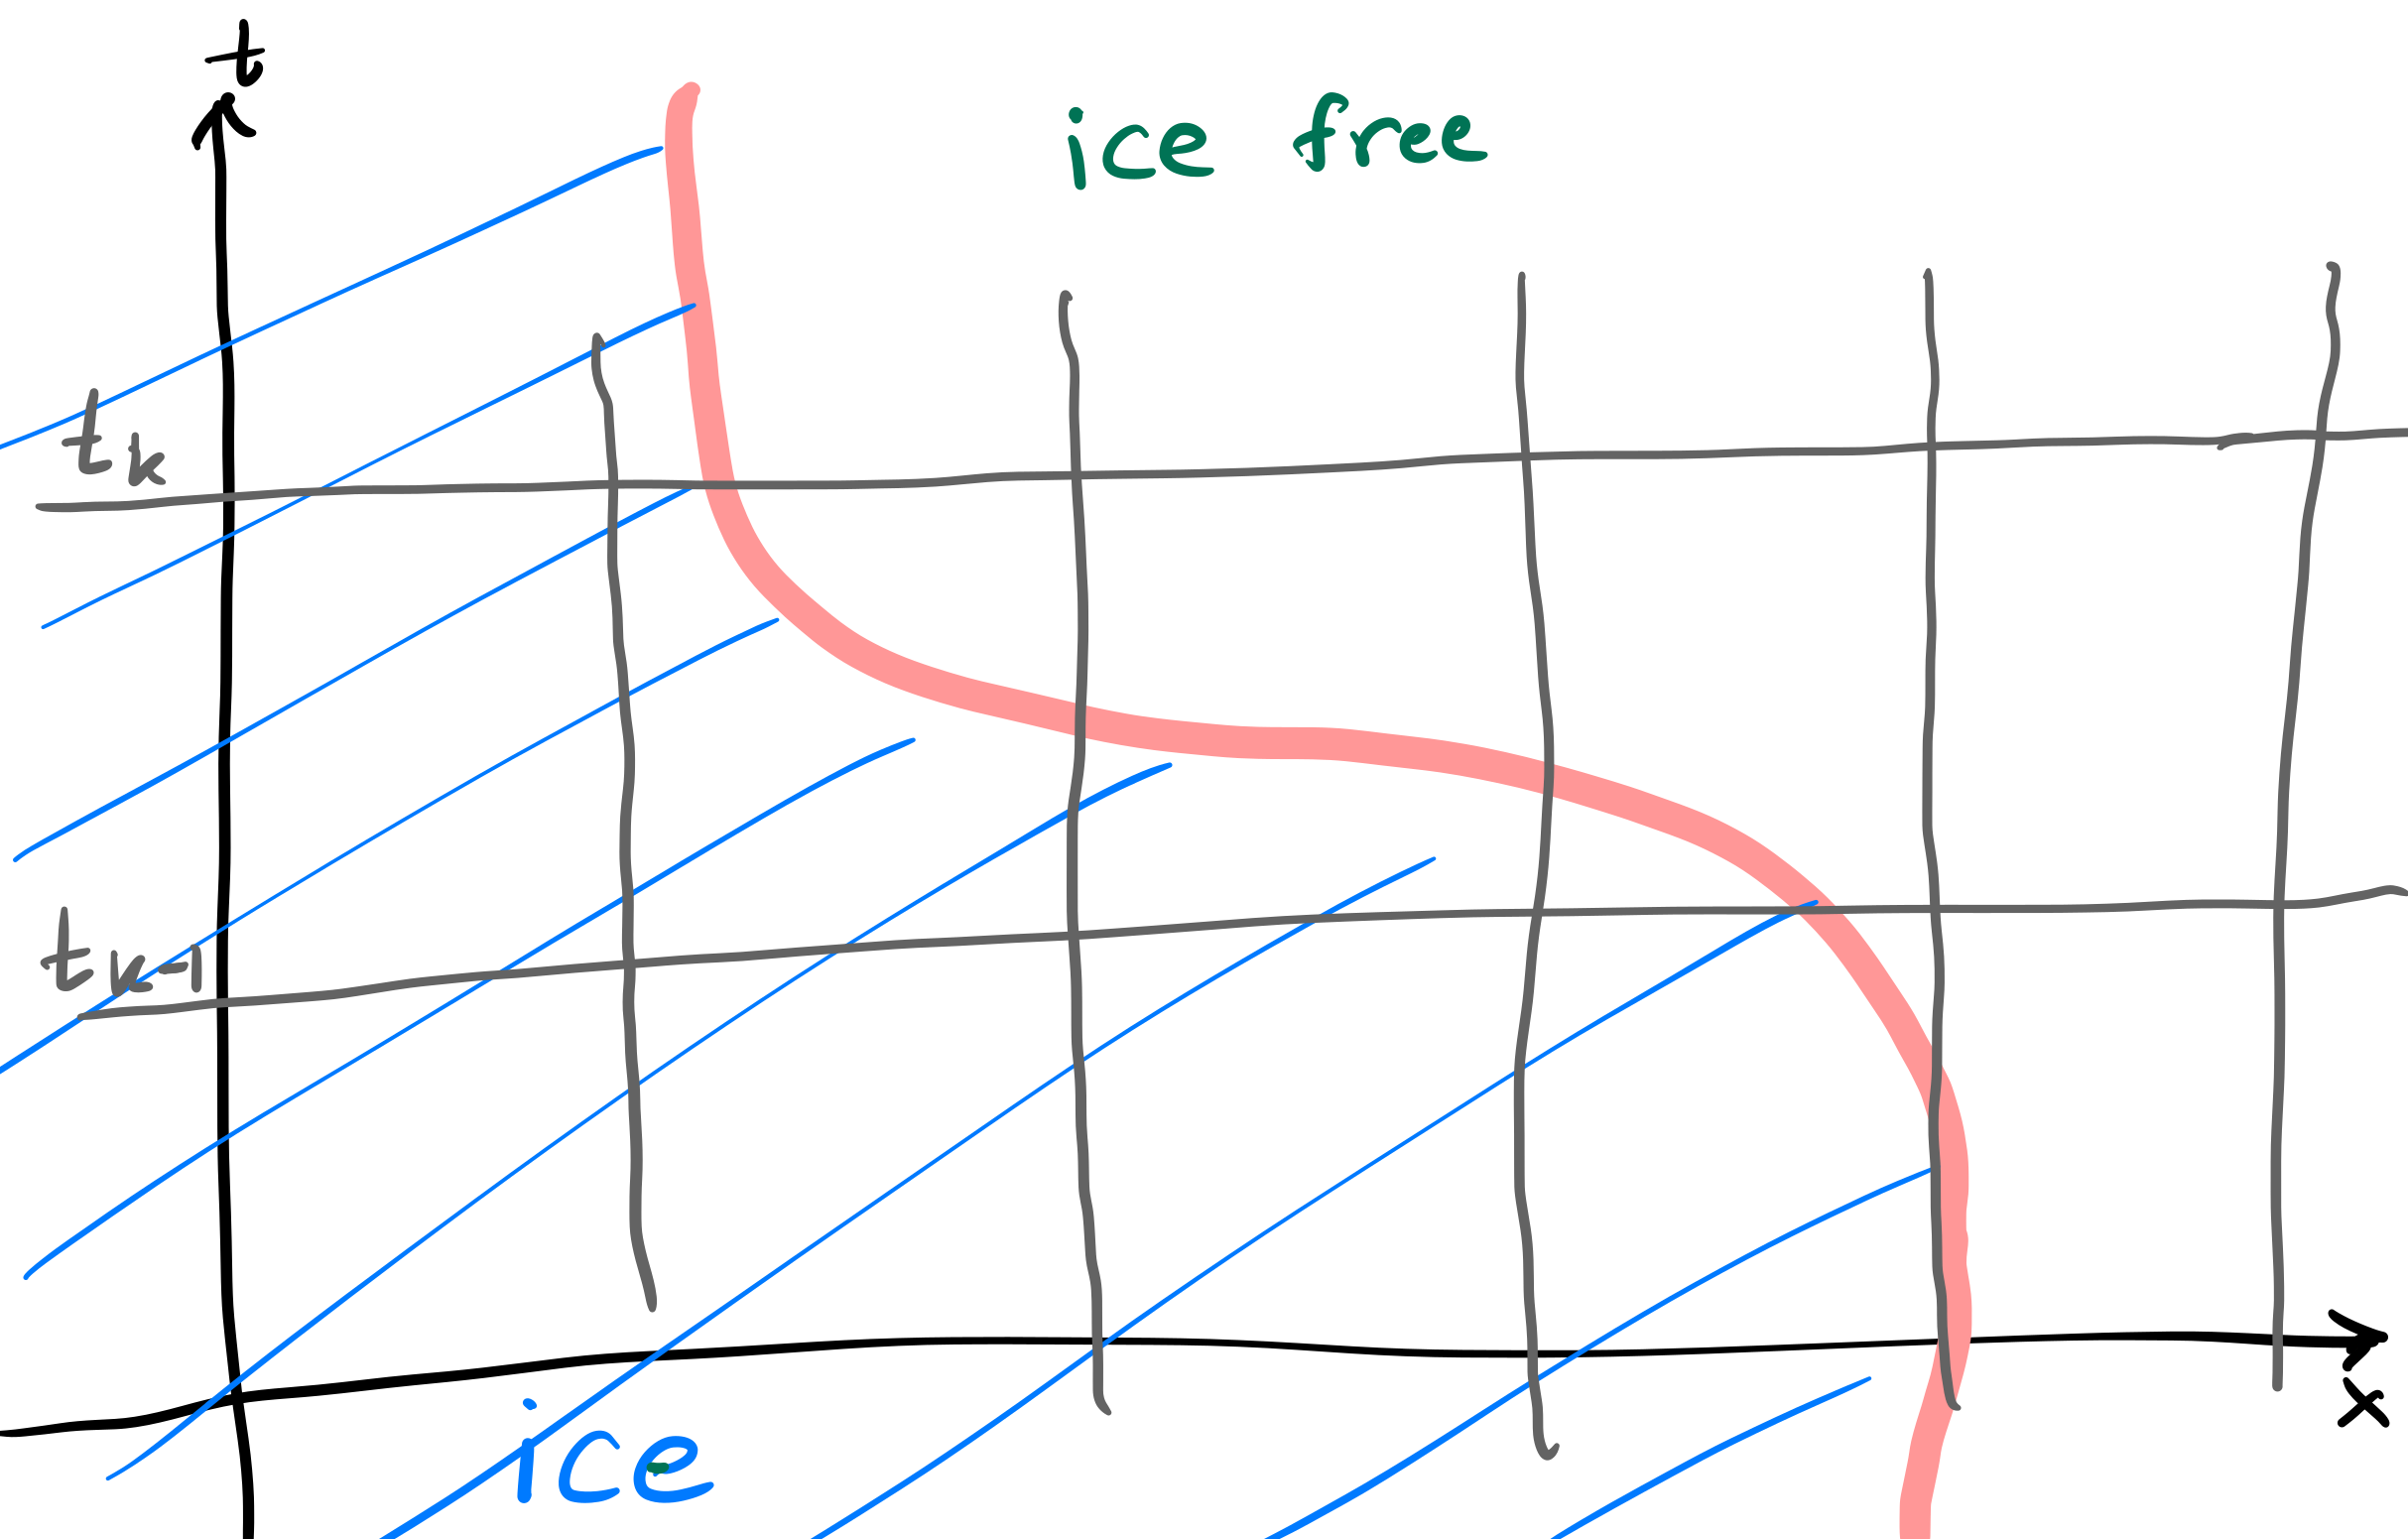
\includegraphics[width=0.75\textwidth]{smbcells}
\end{center}

\bigskip
{\footnotesize \emph{see finite element considerations in} (Bueler 2024)}
\end{frame}


\begin{frame}{benefit 3: mathematical ignorance}

what equations and inequalities, \emph{precisely and mathematically}, determine the evolution of the glaciated area, when using Stokes dynamics?

\bigskip

\begin{center}
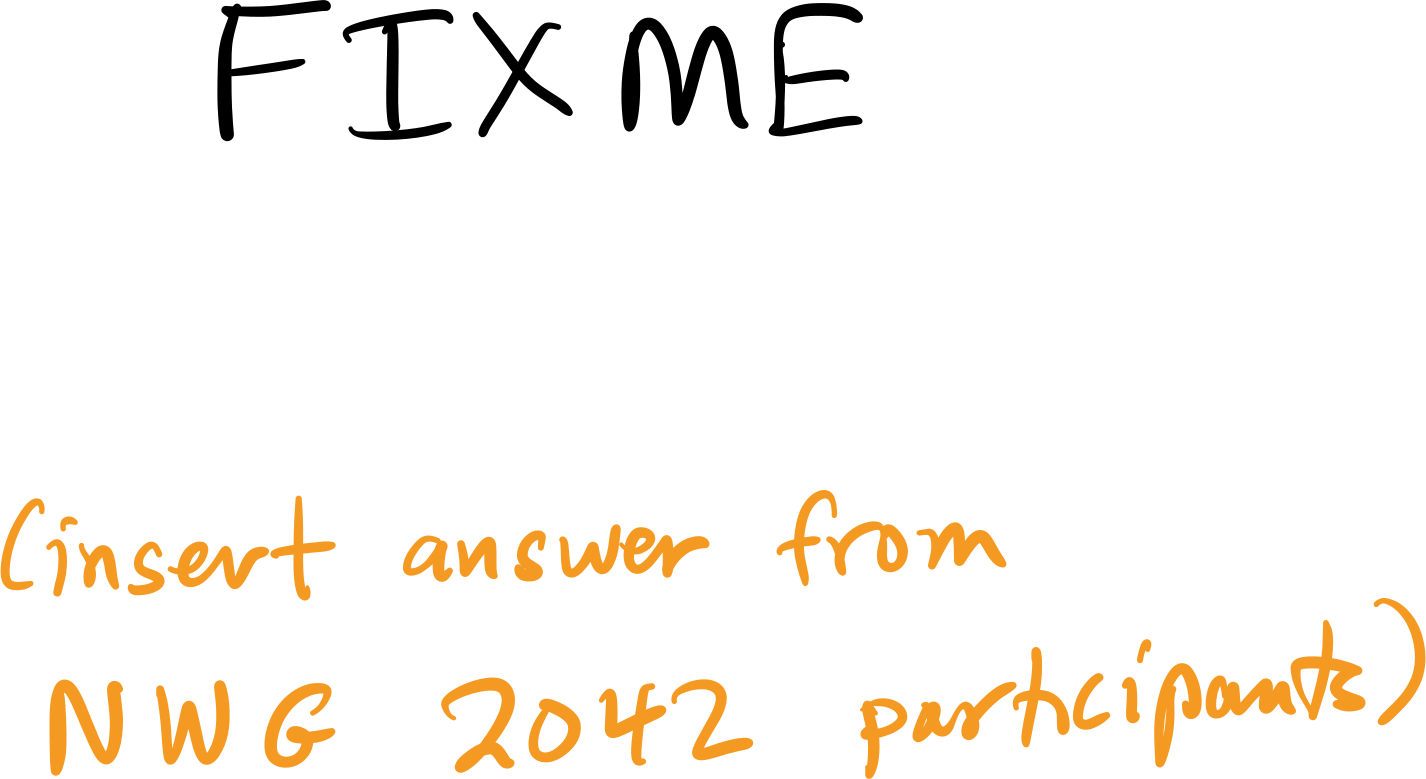
\includegraphics[width=0.5\textwidth]{fixme2042}
\end{center}

\bigskip
\viewin{(Calvo et al 2003) \emph{and} (Jouvet \& Bueler 2012), \emph{but for SIA}}

{\footnotesize \emph{needs fixed-domain Stokes well-posedness from e.g.} (Jouvet \& Rappaz 2011)}

{\footnotesize \emph{see conjectures in} (Bueler 2024)}
\end{frame}


\end{document}
